% Created 2016-09-12 Mon 12:54
\documentclass[presentation]{beamer}
\usepackage[utf8]{inputenc}
\usepackage[T1]{fontenc}
\usepackage{fixltx2e}
\usepackage{graphicx}
\usepackage{grffile}
\usepackage{longtable}
\usepackage{wrapfig}
\usepackage{rotating}
\usepackage[normalem]{ulem}
\usepackage{amsmath}
\usepackage{textcomp}
\usepackage{amssymb}
\usepackage{capt-of}
\usepackage{hyperref}
\usetheme{default}
\author{Paul M. Magwene}
\date{}
\title{Describing univariate distributions}
\definecolor{links}{HTML}{2A1B81}
\hypersetup{colorlinks,linkcolor=,urlcolor=magenta}
\useinnertheme[shadow,outline]{chamfered}
\usecolortheme{beaver}
\beamertemplatenavigationsymbolsempty
\usefonttheme{professionalfonts}

\let\digamma\relax
\usepackage[scale=0.85,stdmathitalics=true,romanfamily=casual]{lucimatx}

\usepackage[scaled=0.85]{zi4}  % inconsolata font
\renewcommand*\familydefault{\ttdefault}

\usefonttheme[stillsansseriftext]{serif}


\institute[Duke]{Department of Biology}
\hypersetup{
 pdfauthor={Paul M. Magwene},
 pdftitle={Describing univariate distributions},
 pdfkeywords={},
 pdfsubject={},
 pdfcreator={Emacs 24.5.1 (Org mode 8.3.5)}, 
 pdflang={English}}
\begin{document}

\maketitle
\definecolor{bg}{rgb}{0.95,0.95,0.95}

\begin{frame}[label={sec:orgheadline1}]{Overview}
\begin{itemize}
\item Terminology for describing univariate distributions
\item Measures of location (centrality)
\item Measures of dispersion (spread)
\end{itemize}
\end{frame}

\begin{frame}[label={sec:orgheadline2}]{Population}
Population -- A population is a collection of objects, individuals, or observations about which we intend to make general statements.

Examples: 

\begin{itemize}
\item The height of American males older than 25 years of age.
\item Number of mitochondrial 12S-rRNA haplotypes in the human population
\item Number of loblolly pine trees per km2 in North Carolina
\end{itemize}
\end{frame}

\begin{frame}[label={sec:orgheadline3}]{Sample / Random Sample}
A sample is a subset of the population.

A Random Sample is a sample that is chosen in such a way as to reflect the
uncertainty of observations in a population.
\end{frame}


\begin{frame}[label={sec:orgheadline4}]{Types of data}
\begin{itemize}
\item Categorical or Nominal -- labels matter but no mathematical notion of order or distance
\begin{itemize}
\item Sex: Male / Female
\item Species
\end{itemize}

\item Ordinal data -- order matters but no distance metric 
\begin{itemize}
\item Juvenile, Adult
\item Small, Medium, Large
\item Muddy, Sandy, Gravelly
\end{itemize}

\item Discrete, Integer, Counting
\begin{itemize}
\item Number of vertebrae in a snake
\item Number of pine trees in a specified area
\item Number of heart beats in a minute
\item Number of head bobs during courtship display
\end{itemize}

\item Continuous
\begin{itemize}
\item Body mass
\item Length of right femur
\item Duration of aggressive display
\end{itemize}
\end{itemize}
\end{frame}

\begin{frame}[label={sec:orgheadline5}]{Interval vs Ratio scales}
\begin{itemize}
\item Interval scales -- have meaningful order and distance metrics, but don't usually have a meaningful zero value, so computing ratios don't make sense

\item Ratio scales -- have a meaningful order, distance metrics, and zero value.
\end{itemize}
\end{frame}


\begin{frame}[label={sec:orgheadline6}]{Statistic}
A statistic is a numerical value calculated by applying a function (algorithm) to the values of the items of a sample 
\end{frame}


\begin{frame}[fragile,label={sec:orgheadline7}]{Example data set: butterfat data}
 We'll use a data set that records the butter fat percentage in milk from 120 Canadian dairy cows (Sokal and Rohlf, Biometry, 4th ed)

\begin{itemize}
\item See the link on the course wiki for \texttt{butterfat.csv}
\item Load \texttt{butterfat.csv} using the \texttt{read.csv} function
\end{itemize}
\end{frame}


\begin{frame}[fragile,label={sec:orgheadline8}]{Generate a histogram}
 Using the \texttt{ggplot2} library, generate a histogram for the butterfat data set.

\begin{figure}[htb]
\centering
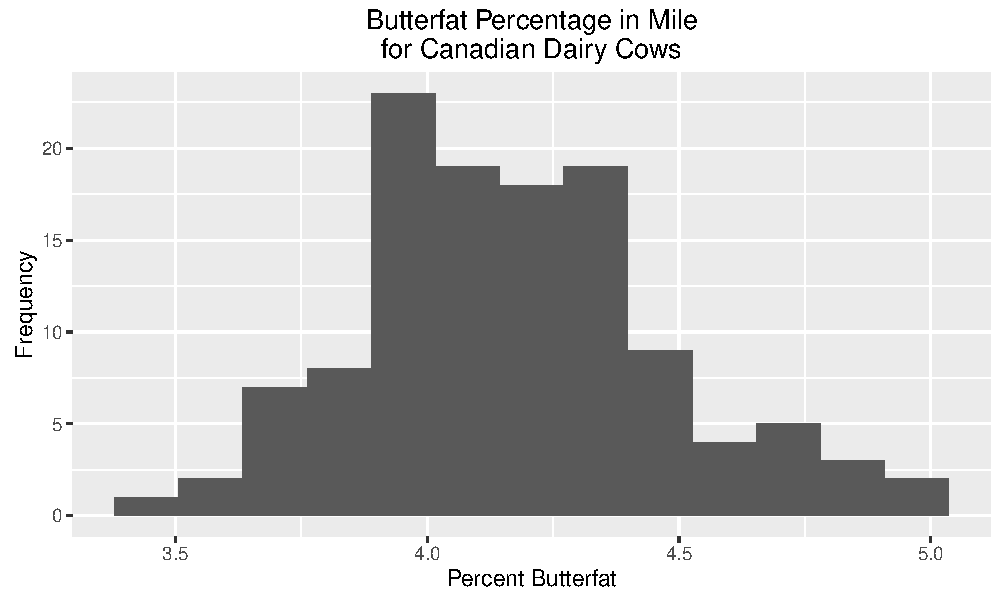
\includegraphics[height=0.5\textheight]{butterfat-hist.pdf}
\caption{Histogram of butter fat percentage from 120 Canadian cows.}
\end{figure}
\end{frame}




\section{Measures of location}
\label{sec:orgheadline14}
\begin{frame}[label={sec:orgheadline9}]{Mean}
\begin{itemize}
\item Most common measure of location
\item Measure of location that minimizes the sum of the squared deviations around it
\item Statistical measure of location that has the smallest standard error (to be defined later)
\item Physical analogy: If we think of observations as points of mass on a line, the mean is the center of mass (balance point)
\end{itemize}

Let \(X = \{x_1, x_2, \ldots, x_n\}\). The mean of \(\mathbf{x}\) is:

\[
\overline{X}= \frac{1}{n} \sum_{i=1}^n x_i 
\]
\end{frame}


\begin{frame}[label={sec:orgheadline10}]{Median}
\begin{itemize}
\item The middle point of a frequency distribution
\item The value of the variable that has an equal number of items on either side of items
\end{itemize}

The median is a \uline{robust} estimator of location. Robust statistics are those that are not strongly affected by outliers our violations of model assumptions.  
\end{frame}

\begin{frame}[label={sec:orgheadline11}]{Robustness of median: Example}
Changes in estimates of location when three outlier values (8, 10, 15) are added to butterfat data.
\end{frame}

\begin{frame}[label={sec:orgheadline12}]{Mode}
\begin{itemize}
\item The most common value (or interval) in a distribution
\item Unimodal, bimodal, multi-modal
\end{itemize}

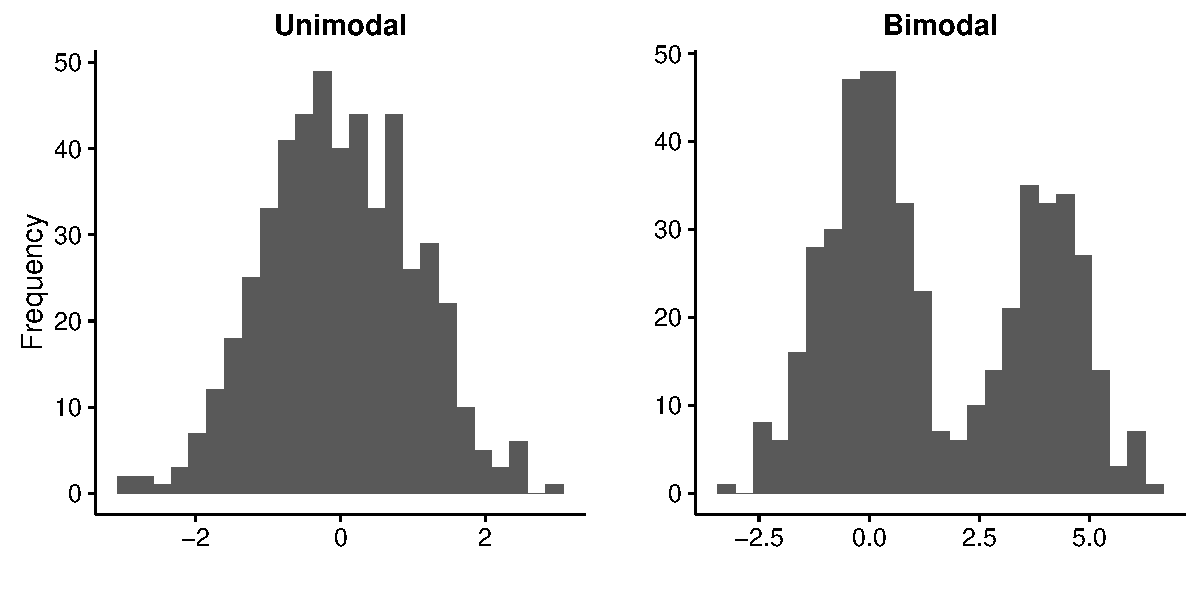
\includegraphics[width=.9\linewidth]{unimodal-and-bimodal.pdf}
\end{frame}

\begin{frame}[label={sec:orgheadline13}]{Some other ``means''}
\alert{Weighted mean} -- useful when there is some a priori notion of weight or importance for different observations
\[
\overline{X}_w = \frac{1}{(\sum^n w_i)} \sum^n w_i x_i
\]
where the \(w_i\) represent the weights attached to each observation.

\alert{Geometric mean} -- most often used to study proportional growth (populations, tissues, organs, etc)
\[
GM_X = \sqrt[n]{\prod^n x_i}
\]

\alert{Harmonic mean} -- rarely used in biology.
\[
HM_X = \frac{1}{n}\sum^n \frac{1}{x_i}
\]
\end{frame}



\section{Measures of dispersion}
\label{sec:orgheadline24}
\begin{frame}[label={sec:orgheadline15}]{Range}
\begin{itemize}
\item The difference between the largest and smallest items in a sample
\end{itemize}

\[
\max(\mathbf{x}) - \min(\mathbf{x})
\]
\end{frame}

\begin{frame}[label={sec:orgheadline16}]{Deviates}
\alert{Deviate} -- the difference between an observation and the mean; can be negative or positive. Units same as the \(x_i\).
\[
x_i - \overline{X}
\]

\alert{Squared deviate} -- the square of a deviate; always \(\geq 0\) (units\(^2\)).
\[
(x_i - \overline{X})^2
\]

\alert{Sum of squared deviations} -- the sum of all the squared deviations in a sample (units\(^2\)). 
\[
\sum_{i=1}^n (x_i - \overline{X})^2
\]
\end{frame}

\begin{frame}[label={sec:orgheadline17}]{Variance and standard deviation}
\alert{Variance} -- the mean squared deviation (units\(^2\)).
\[
\sigma_X^2 = \frac{1}{n} \sum_{i=1}^n (x_i - \overline{X})^2 
\]

\alert{Standard deviation} -- the square root of the variance (units same as the \(x_i\)).
\[
\sigma_X = \sqrt{\frac{1}{n} \sum_{i=1}^n (x_i - \overline{X})^2}
\]

The above are the \uline{population} variance and standard deviation.  
\end{frame}


\begin{frame}[label={sec:orgheadline18}]{Sample estimators of variance and standard deviation}
The \emph{unbiased} \uline{sample} estimators of the variance and standard deviation are given by:
\begin{equation*}
\begin{split}
\mbox{Variance:}\qquad & s_X^2 = \frac{1}{n-1} \sum_{i=1}^n (x_i - \overline{X})^2 \\
\mbox{Standard deviation:}\qquad & s_X = \sqrt{\frac{1}{n-1} \sum_{i=1}^n (x_i - \overline{X})^2}
\end{split}
\end{equation*}

\alert{You almost always want to use the sample estimators of variance and standard deviation.}
\end{frame}

\begin{frame}[label={sec:orgheadline19}]{Standard deviation rules of thumb}
If data are normally distributed:

\begin{itemize}
\item Approximately 68\% of observations fall within 1 standard deviation about the mean
\item Approximately 95\% of observations fall within 2 standard deviations about the mean
\item Approximately 99.7\% of observations fall within 3 standard deviations about the mean
\end{itemize}

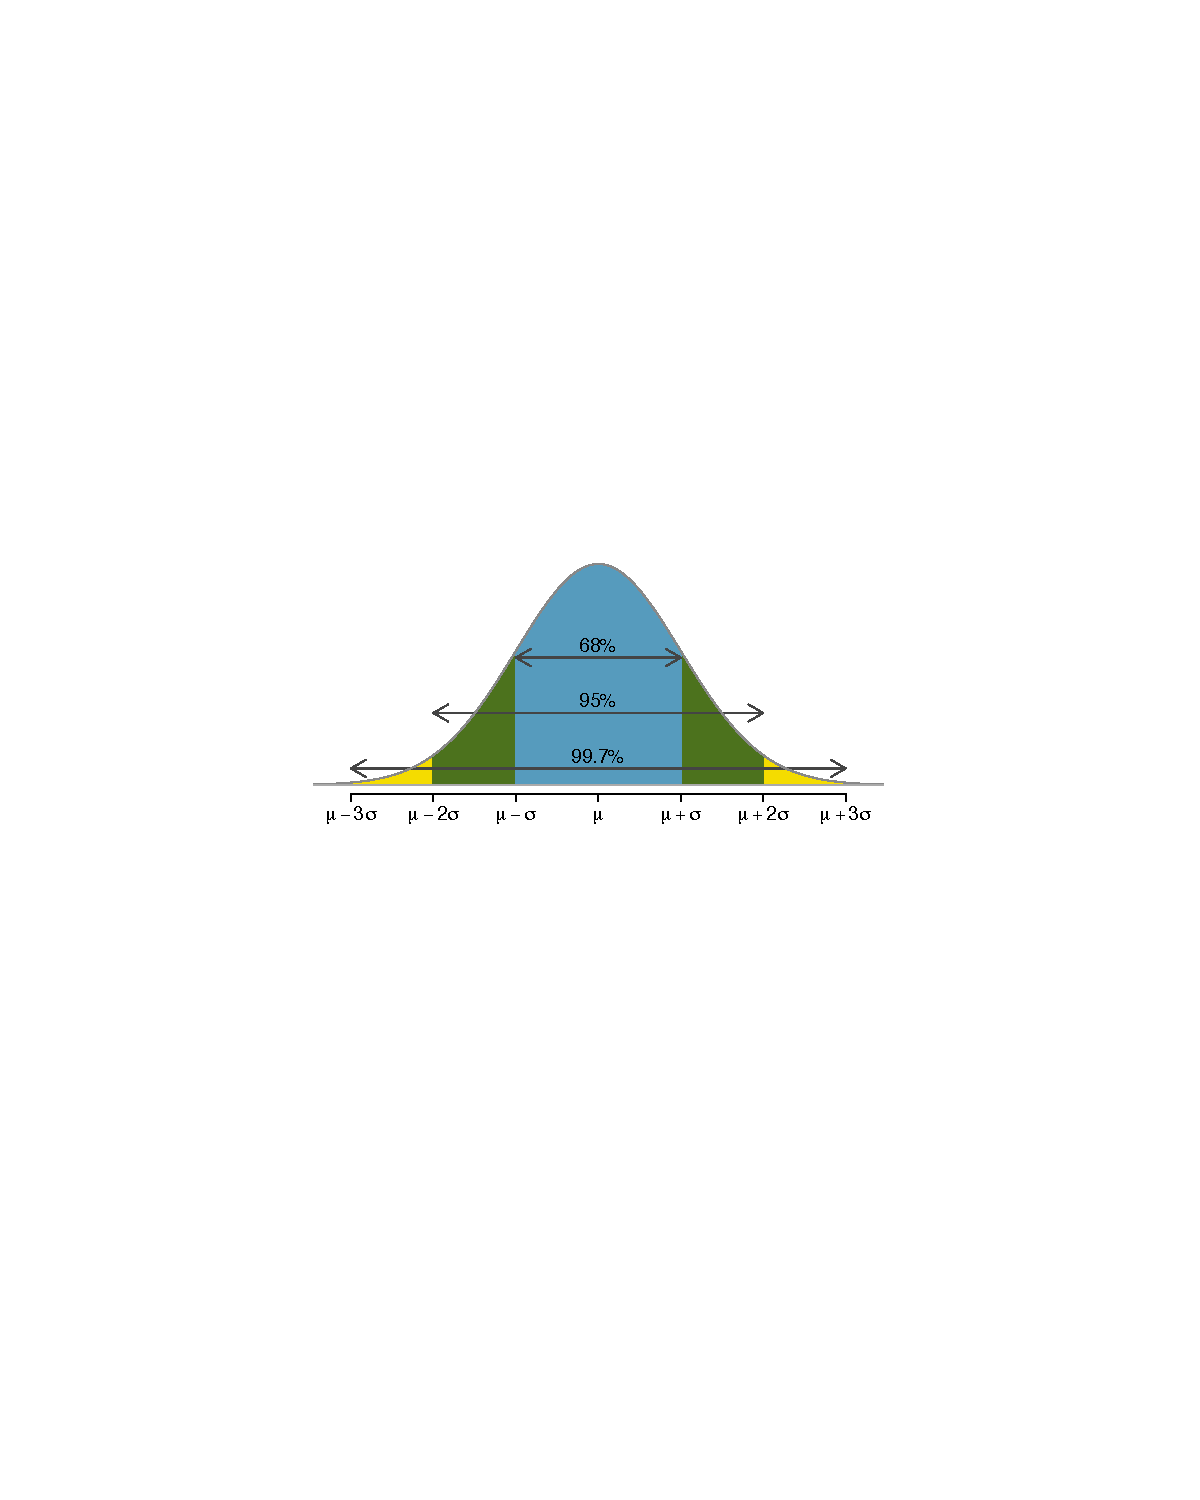
\includegraphics[width=.9\linewidth]{sd-rule-thumb.pdf}
\end{frame}

\begin{frame}[label={sec:orgheadline20}]{Coefficient of variation}
\begin{itemize}
\item Standard deviation expressed as percentage of mean
\item Unitless measure
\end{itemize}

\[
V = \frac{s_X \times 100}{\overline{X}}
\]
\end{frame}



\begin{frame}[label={sec:orgheadline21}]{Quantiles, quartiles, interquartile range}
\begin{itemize}
\item \alert{Quantiles} -- points that will divide a frequency distribution into equal sized groups
\begin{itemize}
\item quartiles -- points dividing a distribution into 4 equal groups
\item deciles -- points dividing a distribution into 10 equal groups
\item percentiles -- points dividing a distribution into 100 equal groups
\end{itemize}
\item \alert{Interquartile range (IQR)}-- range of values that captures the central 50\% of the distribution 
\begin{itemize}
\item Q1 = lower quartile, Q3 = upper quartile
\end{itemize}
\end{itemize}
\end{frame}


\begin{frame}[label={sec:orgheadline22}]{Boxplots typically depict information about quartiles}
\begin{figure}[htb]
\centering
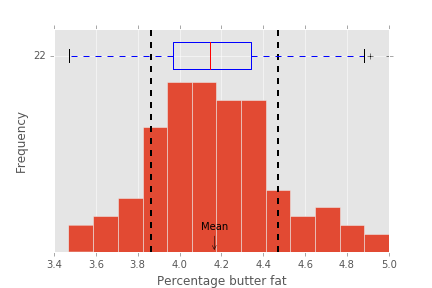
\includegraphics[width=.9\linewidth]{butterfat-hist-boxplot.png}
\caption{Histogram of butterfat data set, with superimposed boxplot.}
\end{figure}
\end{frame}



\begin{frame}[label={sec:orgheadline23}]{Median absolute deviation (MAD)}
\begin{itemize}
\item A robust estimator of dispersion
\end{itemize}

\[
\mathrm{MAD}(X) = \mathrm{median}(|x_i - \mathrm{median}(X)|) 
\]

For normal distribution, \(\sigma_X \approx 1.486 \times \mathrm{MAD}(X)\). 
\end{frame}


\section{Skewness}
\label{sec:orgheadline26}
\begin{frame}[label={sec:orgheadline25}]{Skewness}
\begin{itemize}
\item Skewness describes asymmetry of distributions
\end{itemize}

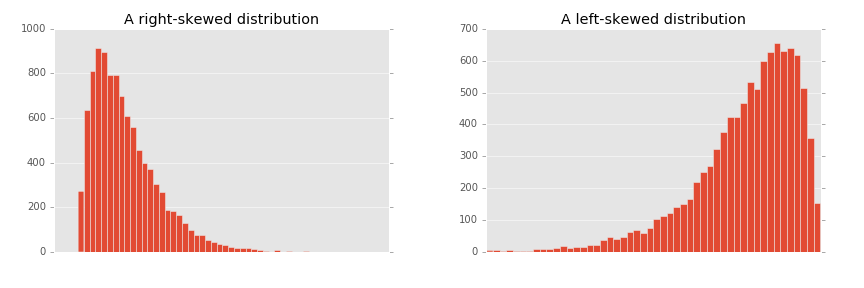
\includegraphics[width=.9\linewidth]{skewed-distributions.png}

Common measure of skewness:

\[
\mbox{skewness} = E\left[\left(\frac{(x - \mu}{\sigma}\right)^3\right]
\]
\end{frame}
\end{document}